\makeatother
\setlength\tabcolsep{1mm}
\renewcommand\arraystretch{1.3}
\newcounter{FiguraCap4}
\renewcommand\theFigura{\arabic{FiguraCap4}}
\newcounter{TablaCap4}
\renewcommand\theTabla{\arabic{TablaCap4}}

\chapter{Diseño}
\label{capitulo4}
	En este capítulo se propone una solución que respeta los requerimientos que se especificaron
		durante el capítulo anterior. Además se describe el funcionamiento de la herramienta propuesta identificando los componentes que
		participan en dicho proceso. También se explica la arquitectura de la aplicación con la función de cada una de sus
		componentes. Finalmente se detalla el modelo de datos creado para la base de datos.
	
	\section{Contexto para el uso del sistema} 
	Por medio del sistema propuesto es posible ingresar información de seguridad, correlacionarla
		con información existente en el sistema, y, luego de ser sanitizada, compartirla con organizaciones socias.
	
	
	\bigskip
	
	El sistema ha sido diseñado para que sea utilizado por grupos de seguridad. Se busca que
		dichos grupos puedan compartir información de incidentes de seguridad representada con el lenguaje STIX y que sea
		distribuida utilizando TAXII. El diseño y desarrollo de STIX y TAXII ha sido realizado por MITRE con el apoyo de la
		comunidad. El intercambio de información da a las organizaciones la posibilidad de identificar adecuadamente las
		amenazas dando evidencias específicas de su existencia.
	
	
	\bigskip
	
	Se busca que la herramienta ayude a solucionar algunas de las problemáticas a las que se
		enfrentan las organizaciones durante el intercambio de información de seguridad. Dichas problemáticas se abordan
		durante el capítulo de análisis.
	
	\section{Componentes del sistema}
	
	\bigskip
	
	En esta sección se presenta el sistema diseñado, mostrando en la figura \ref{fig.arquitecturasistema} su arquitectura. El sistema busca darle a las organizaciones la capacidad de intercambiar
		información de seguridad de forma automática. Se busca integrar a RTIR dicha capacidad utilizando las herramientas
		mencionadas anteriormente.
	
	\bigskip
	
	Para ello se busca extender RTIR para que el usuario ingrese la información al sistema, con
		dicha información se crea un ticket en RTIR y a su vez se envía a TAXII App para crear una representación utilizando
		STIX. El sistema TAXII es un desarrollo nuevo que utiliza librerías provistas por MITRE, estas son utilizadas para
		representar e intercambiar la información.
	
	
	\bigskip
	
	\begin{figure}[ht!]
		\centering
		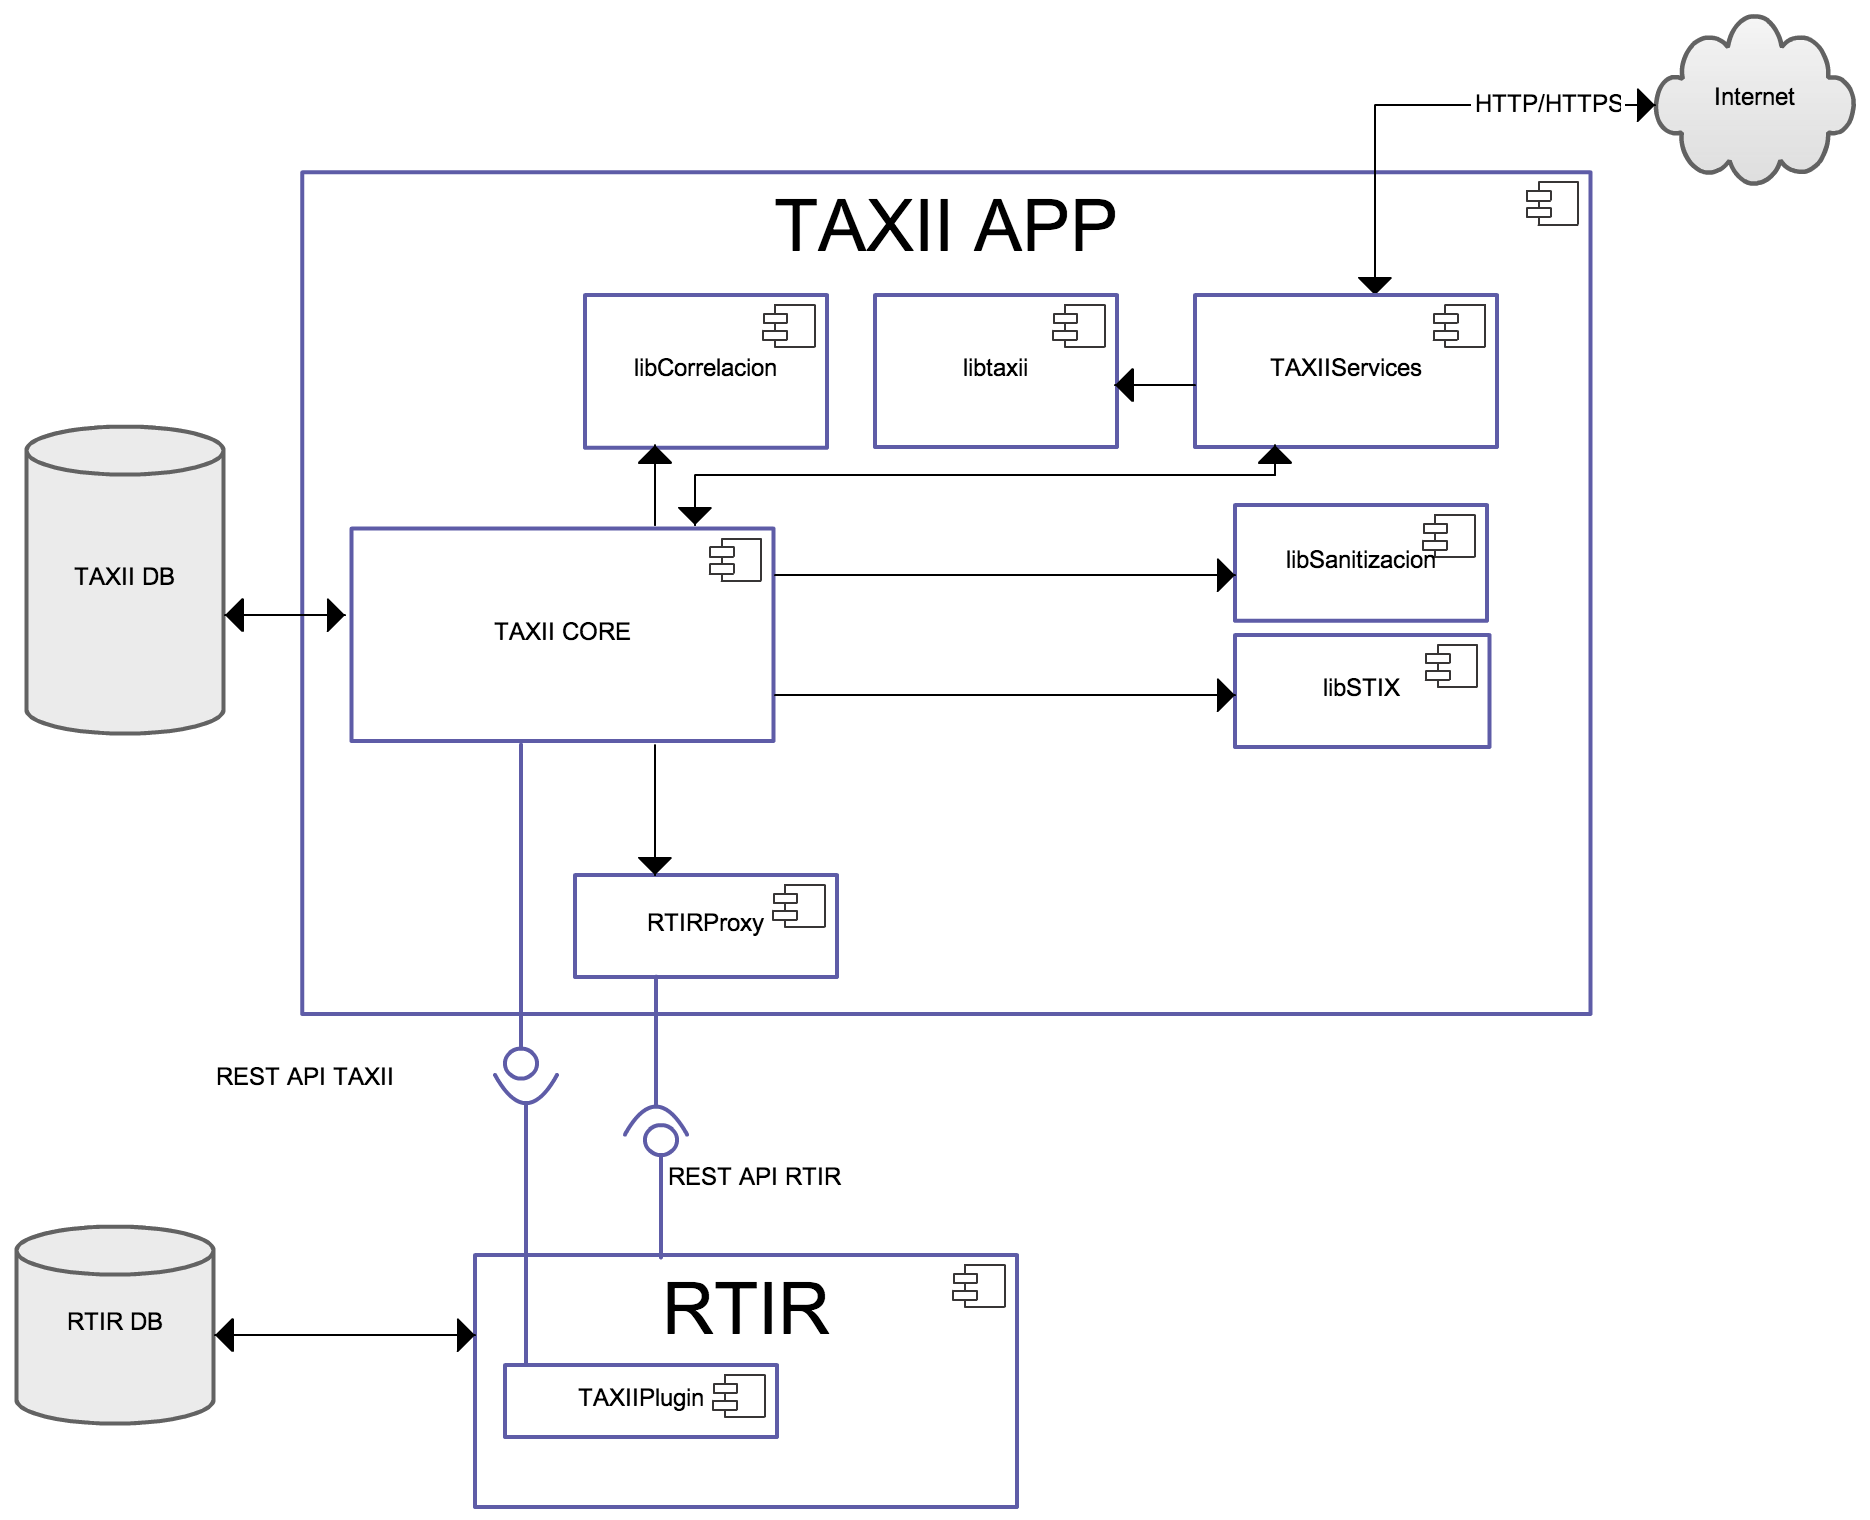
\includegraphics[width=5.7638in,height=4.6846in]{Diseno21-img/Diseno21-img003.png} 
		\caption{Arquitecture del sistema}	
		\label{fig.arquitecturasistema}
	\end{figure}
	\bigskip
	
	
	\section{Aspectos generales de las componentes del sistema}
	
	

	En la figura \ref{fig.arquitecturasistema} se pueden ver dos bases de datos: TAXII DB y RTIR DB. A su vez se cuenta con dos
		aplicaciones: RTIR y TAXII App. RTIR es la aplicación para manejo de incidentes desarrollada por la empresa
		Bestpractial \cite{bp} y elegida para el desarrollo de este proyecto. TAXII App es una aplicación nueva que será
		desarrollada durante el proyecto y se encarga de representar la información de forma estructurada e intercambiar dicha
		información de seguridad.
    \bigskip
	
	La aplicación RTIR recibe datos ingresados por un analista y los transmite a la aplicación
		TAXII App. Para realizar dicha transmisión es necesario extender RTIR para consumir una API REST publicada por el
		cliente TAXII. La aplicación RTIR también puede recibir de la aplicación TAXII App información, la cual puede
		estar relacionada a tickets existentes y contener soluciones a problemas, identificación de atacantes, etc.
	
	
	\bigskip
	
	La aplicación TAXII recibe datos de RTIR así como también de organizaciones socias, en un
		futuro se podría dar la posibilidad de que la aplicación TAXII recibiera datos de sensores que se encuentren en la red
		de la organización. Luego de que los datos son recibidos y almacenados se correlacionan con los ya existentes en por TAXII App. De la
		correlación se pueden obtener soluciones a problemas encontrados, información sobre ataques realizados, identificación
		de atacantes, etc. En caso de que exista información de utilidad se pueden ingresar notas a tickets o relacionar
		tickets existentes en el RTIR.\\
		\bigskip
	También se podría compartir información con otras organizaciones para colaborar en la lucha
		contra amenazas. Para realizar dicho intercambio se representa la información utilizando STIX y luego se intercambia
		utilizando TAXII. Se utilizan librerías provistas por MITRE para realizar la representación y el intercambio de la
		información.
	
	
	\bigskip
	
	La aplicación TAXII App es independiente de la aplicación RTIR, siendo posible reemplazar esta
		última por otra herramienta con funcionalidades similares. Es deseado que la herramienta que pueda reemplazar a RTIR
		pueda ser extendida de forma de invocar a las funcionalidades desarrolladas en TAXII App. Además deberia contar con un método por el
		cual la TAXII App pueda utilizar la funcionalidades de la herramienta que sustituya a RTIR.
	
	\subsection{RTIR}
	Este componente presenta las funcionalidades originales de la herramienta RTIR con un agregado
		específico implementado para este proyecto. RTIR es el componente de la aplicación encargado de realizar el manejo de
		los incidentes. Se agrega una extensión que permite invocar una API REST en la aplicación TAXII.
	\bigskip
	
	RTIR cuenta con su propia base de datos, RTIR DB, a la cual solo accede la componente RTIR, que no será modificada para la realización de este proyecto.
	
	
	\bigskip
	
	\subsection{TAXII App}
	
	\bigskip
	
	La segunda componente presente es TAXII App, está compuesta por otros componentes
		implementados durante el proyecto así como por librerías provistas por MITRE. Los componentes provistos por MITRE son
		libTAXII y libSTIX, a estos no se le realizarán cambios debido a que cuentan con las funcionalidades necesarias para
		llevar a cabo el proyecto. En el caso de libSTIX permite representar la información recibida por medio del lenguaje
		STIX, por otro lado libTAXII permite la creación de mensajes TAXII para que estos sean intercambiados. El componente
		TAXII App utiliza los componentes TAXIICore, RTIRProxy y TAXIIServices, estos son implementados durante el transcurso
		del proyecto.
	
	\subsubsection{libTAXII}
	libTAXII \cite{libtaxii} es una librería que provee una representación de objetos de los mensajes TAXII, cuenta además
		con una serie de métodos para el manejo de dichos mensajes. Provee clientes para http y https. La librería se utiliza
		para generar los mensajes y dispone métodos para transformarlos a xml, estos xml son utilizados en los intercambios
		entre cliente y servidor.
	
	\subsubsection{libSTIX}
	libSTIX es una librería provista por MITRE para parsear, manipular y generar contenido STIX.
	
	\subsubsection{RTIRProxy}
	RTIRProxy es la componente de TAXII App encargada de integrarse con RTIR, para ello consume la
		API REST provista por RTIR para el manejo de tickets. Por ser una API REST la comunicación está encapsulada en el
		protocolo http. Ésta componente busca que se tenga independencia de RTIR permitiendo el uso de otro sistema en su
		lugar. Lo que se logra es que si otro sistema tiene una API
		o un método de integración distinto al de RTIR se re implemente esta componente. La única premisa que se debe cumplir
		es que la interfaz con la cual se comunique TAXIICore se mantenga. Dentro de dichos tipos de integración podría
		encontrarse otra API REST o web services con SOAP.
	
	\subsubsection{TAXIICore}
	Es necesario que este componente tenga una interfaz de web services REST para realizar la
		comunicación con el RTIR. En dicha interfaz se deben dar operaciones para realizar el alta de información, obtener
		información de servicios publicados por contrapartes, enviar y recibir información de seguridad entre contrapartes.\\
		\bigskip

	Además debe proveer una interfaz para que la componente TAXIIServices envíe la información
		recibida en la aplicación TAXII, en dicha interfaz se deben recibir tanto paquetes STIX así como información adicional
		utilizada por el protocolo TAXII. \\
	\bigskip	
	La información tomada de la base de datos es enviada en forma de objetos STIX junto a las
		políticas definidas por los administradores para que sea sanitizada. Luego de que la información es sanitizada es
		enviada a TAXIIServices para que sea compartida con las organizaciones socias.
	
	\subsubsection{libSanitizacion}
	Esta es la componente encargada de realizar la sanitización de la información que se desea
		intercambiar entre los sistemas. Para realizar dicha sanitización se podrían utilizar librerías ya existentes o implementar una
		propia. La componente se alimenta de políticas definidas por los administradores para realizar la
		sanitización.
	
	\subsubsection{libCorrelacion}
	Es la componente encargada de la correlación de los datos del sistema, dicha correlación se
		realiza por medio de políticas ingresadas por los administradores del sistema. La componente ayuda a agrupar datos que
		tengan características similares lo que facilita el trabajo de los analistas y da más valor a la información recibida.
		Se pueden utilizar distintos métodos para realizar las correlaciones y de ahí se desprende la necesidad de que sea un
		componente separado del Core del sistema. Los datos correlacionados son los almacenados en TAXII DB.
	
	\subsubsection{TAXIIServices}
	Esta componente es una implementación de los servicios TAXII como se especifica en \cite{M13} \ y
		\ \cite{M14} 
	
	TAXIIServices provee los siguientes servicios:
	
	\begin{itemize}
		\item \underline{Inbox}: Por medio de este servicio el sistema acepta mensajes enviados por otro cliente
			TAXII en intercambios iniciados por este.
		\item \underline{Poll}: Este servicio es el que utiliza el sistema para consumir datos provenientes de un
			TAXII Data Feed en un cliente TAXII.
		\item \underline{Discovery}: Es el servicio encargado de la comunicación de información referente a la
			disponibilidad y uso de los servicios TAXII en el sistema.
	\end{itemize}
	
	\bigskip
	
	Utiliza la componente libTAXII para crear mensajes TAXII y de esa forma realizar el
		intercambio de documentos STIX recibidos de libSanitizacion. Los mensajes que son recibidos de otros socios son pasados
		a la componente TAXIICore para que sea almacenada y luego correlacionada con datos existentes.
	
	
	\bigskip
	
	\section{Comunicación entre los componentes}
	
	\bigskip
	
	En la comunicación entre RTIR y la aplicación TAXII se utiliza REST (\textit{Representational State
		Transfer}), en este tipo de servicio web se trata de emular \ el protocolo http o algún protocolo similar usando la
		restricción de proveer una interfaz a un conjunto conocido de operaciones estándar (GET, PUT, etc). Se utiliza este
		tipo de servicio web debido a que RTIR provee una API de este tipo.
	
	
	\bigskip
	
	El intercambio entre las distintas organizaciones se realiza por medio de HTTP/HTTPS. Esto se
		debe a que hasta el momento MITRE solo ha especificado el intercambio por medio de dicho protocolo. Se podrían utilizar
		otros protocolos para realizar el intercambio pero sería necesario que MITRE definiera las especificaciones para su
		uso, un ejemplo de ellos podría ser SOAP.

	
	\bigskip
	
	\section{Modelo de datos}
	El modelo de datos diseñado se adapta a las necesidades de TAXII, dichas necesidades están
		definidas en \ \cite{M15}, además se agrega una tabla para realizar el mapeo entre los elementos de RTIR y los elementos
		TAXII intercambiados. En la figura \ref{fig.diagramadedatos} se ve el modelo de datos \ y a continuación se explica cada una de sus
		componentes.
	
	\begin{figure}[ht!]
	\centering
	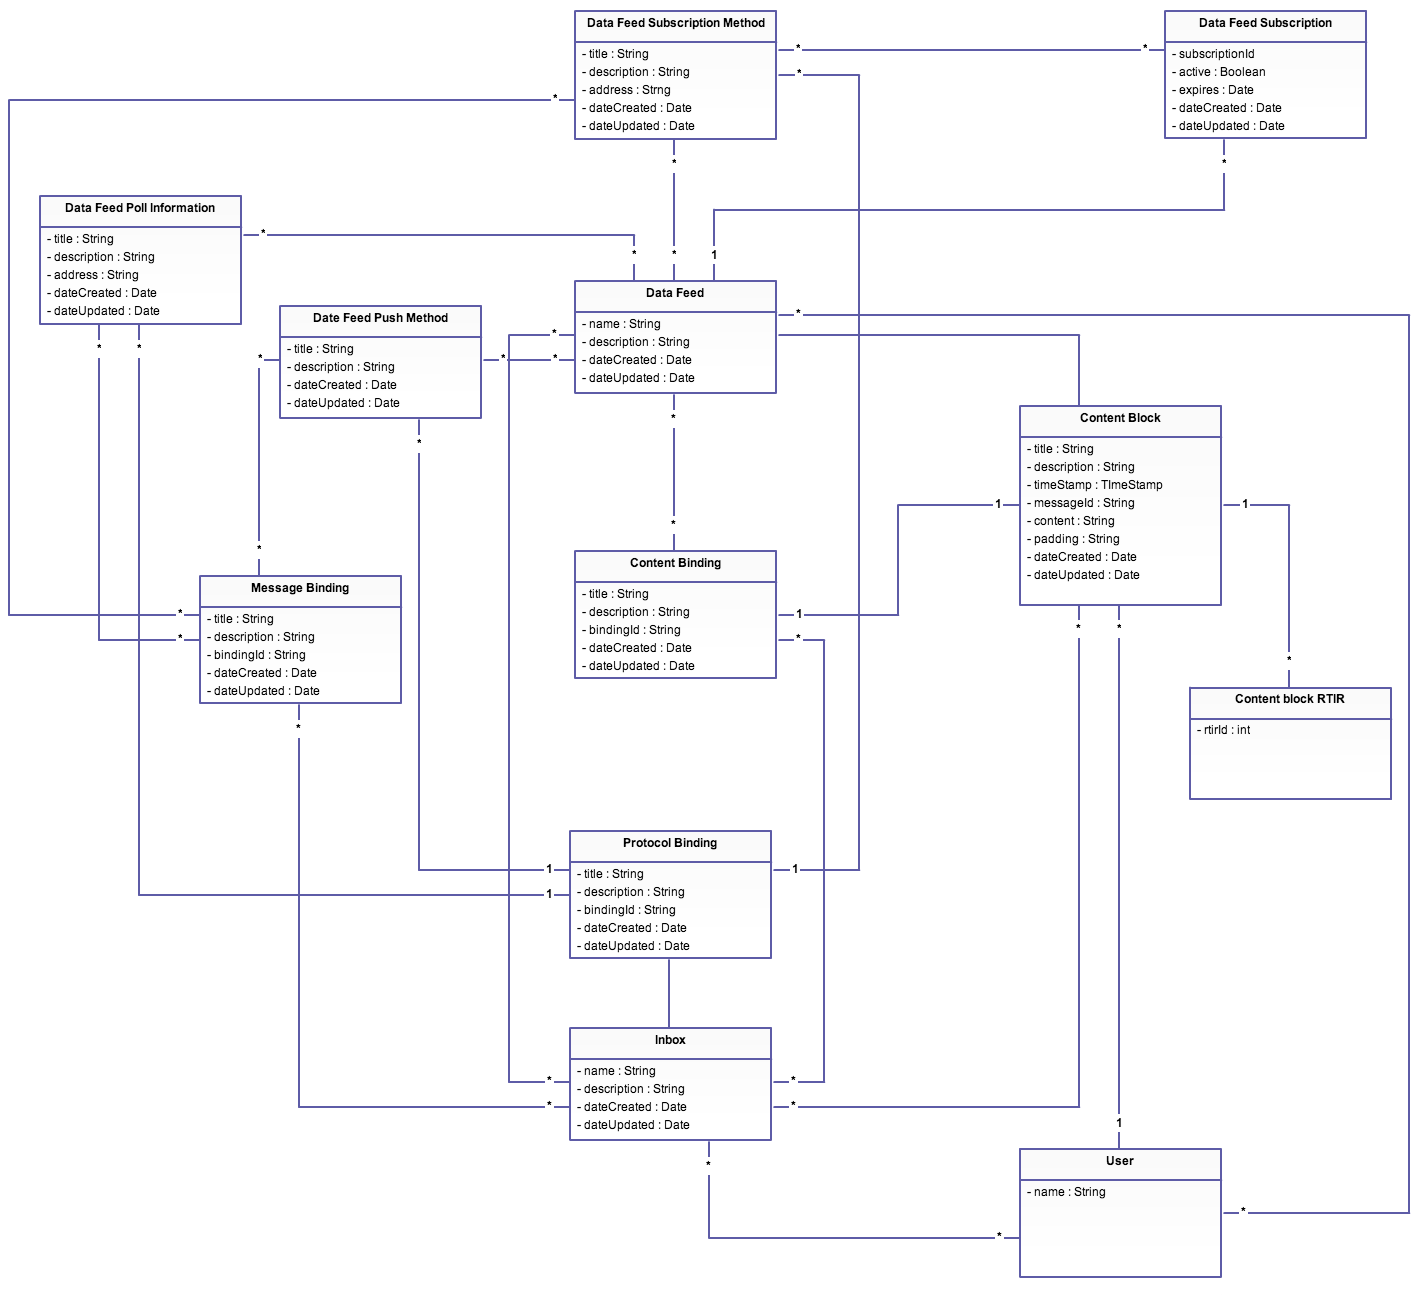
\includegraphics[width=5.7638in,height=5.3126in]{Diseno21-img/Diseno21-img004.png} 
	\caption{Diagrama de datos}
	\label{fig.diagramadedatos}
	\end{figure}
	\bigskip
	
	
	\begin{itemize}
		\item \underline{Protocol Binding}: Es un elemento utilizado para establecer el protocolo de intercambio
			soportado por una implementación de TAXII.
		\item \underline{Content Binding}: Es utilizado para establecer el tipo de contenido soportado para un
			cierto intercambio realizado con TAXII, por ejemplo:
		\textit{Poll},
	\textit{Inbox}, etc.
	\item \underline{Message Binding}: Es utilizado para establecer el tipo de sintaxis para un intercambio
		realizado con TAXII.
	\item \underline{Data Feed Push Method}: Es utilizado para establecer los protocolos que pueden ser
		utilizados para enviar contenido por medio de una subscripción. Esto se utiliza en un mensaje de tipo
	\textit{Feed Information Response}. Es definido en \cite{M14}.
	\item \underline{Data Feed Poll Information}: Tiene la finalidad de establecer los protocolos soportados y
		las direcciones de una fuente de información (\textit{Data
			Feeds}). Es utilizado en los mensajes de \textit{Feed Information
			Response} como se define en \cite{M14}.
	\item \underline{Data Feed Subscription Method}: Es utilizado para identificar el protocolo y la dirección
		de un servicio de \textit{Feed Managment} que pueda procesar las
		subscripciones a fuentes de información TAXII.
	\item \underline{Content Block}: Representa el contenido de los mensajes
\textit{Poll Response }o \textit{Inbox
		Messages}. Es necesario señalar que el campo
\textit{content} representa un mensaje STIX. Dicho mensaje
representa la información de seguridad estructurada, la cual fue representada utilizando el lenguaje STIX.
\item \underline{Data Feed}: Representa una fuente de información TAXII, los usuarios se suscriben a
	dichas fuentes de información para recibir datos que sean de su interés.
\item \underline{Data Feed Subscription}: Representa una subscripción a fuentes de datos TAXII.
\item \underline{Inbox}: Representa un \textit{inbox
	}TAXII, estos son el mecanismo por el cual los consumidores reciben información de otros
	clientes TAXII que nos envían información. La representación permite que un
\textit{inbox} este asociado a ningún o muchas fuentes de datos.

\item \underline{Content Block RTIR}: Representa el nexo entre los contenidos TAXII y los tickets
	existentes en RTIR.
\end{itemize}